% !TeX spellcheck = cs_CZ
%{\tikzset{external/prefix={tikz/FYZII/}}
% \tikzset{external/figure name/.add={ch31_}{}}
%---------------------------------------------------------------------------------------------------
% file fey2ch31.tex
%---------------------------------------------------------------------------------------------------
%=========================== Kapitola Tenzory ======================================================
\setchaptertoc
\chapter{Tenzory}\label{fyz:IIchapXXXI}

  \section{Tenzory polarizovatelnosti}\label{fyz:IIchapXXXIsecI}
    Fyzici mají ve zvyku zvolit nejednodušší příklad nějakého jevu a nazvat jej „fyzikou", přičemž
    komplikovanější příklady nechávají na starosti jiným odvětvím, například aplikované matematice,
    elektroinženýrství, chemii nebo krystalografii. Dokonce i fyzika pevných látek je téměř
    „polofyzikou”, neboť se příliš zajímá o speciální látky. Proto i v těchto přednáškách budeme
    vynechávat spoustu zajímavých věcí. Například jednou z důležitých vlastností krystalů, nebo
    většiny látek, je to, že jejich elektrická polarizovatelnost je v různých směrech různá.
    Nachází-li se látka ve elektrickém poli, které má určitý směr, posunou se mírně náboje atomů a
    vytvoří se dipólový moment. Velikost tohoto momentu silně závisí na směru pole. A to je,
    samozřejmě, určitá komplikace. Ale ve fyzice si to zjednodušujeme a obvykle začínáme se
    speciálním případem, kdy je polarizovatelnost stejná ve všech směrech. Ostatní případy necháváme
    na starosti jiným vědním oborům. Proto v našich dalších úvahách vůbec nebudeme potřebovat to, o
    čem budeme mluvit v této kapitole.
    
    Matematika tenzorů je zvláště užitečná při popisu těch vlastností látek, které závisejí na
    směru, ačkoliv je to jen jeden z příkladů jejího využití. Jelikož většina z vás se nemíní stát
    fyziky, ale budete se zabývat reálným světem, kde věci silně závisejí na směru, budete muset
    dříve či později používat tenzory. Abychom nic nevynechávali, pohovoříme o tenzorech. Chceme,
    aby naše chápání fyziky bylo co nejúplnější. Například náš výklad elektrodynamiky je úplný - tak
    úplný jako libovolný kurz elektřiny a magnetizmu, dokonce i pro fyzikální specializace na vysoké
    škole. Mechanika nebyla úplně ukončena, protože, když jsme ji probírali, nebyly ještě naše
    matematické znalosti na takové úrovni, abychom mohli hovořit o tématech, jako je princip
    nejmenšího účinku, lagranžiány, hamiltoniány atd., které představují elegantnější způsob popisu
    mechaniky. Ale s výjimkou obecné teorie relativity jsme všechny zákony mechaniky probrali. Naše
    elektřina a magnetizmus jsou kompletní a mnoho dalších oblastí je v podstatě uzavřeno. Kvantová
    mechanika přirozeně ne; musíme si něco nechat do budoucna. Ale co je tenzor, musíme vědět už
    nyní. 

    V kapitole \ref{fyz:IIchapXXX} jsme zdůrazňovali, že vlastnosti krystalických látek jsou v
    různých směrech různé, říkáme, že jsou anizotropní. Závislost indukovaného dipólového momentu na
    směru vnějšího elektrického pole je jen jedním z možných příkladů, ale právě ten si vybereme
    jako příklad tenzoru. Předpokládejme, že při daném směru elektrického pole je indukovaný
    dipólový moment objemové jednotky \(\vec{P}\) úměrný intenzitě vnějšího pole \(\vec{E}\). (To je
    dobrá aproximace pro většinu látek, pokud \(\vec{E}\) není příliš velké.) Konstantu úměrnosti
    označíme \(\alpha\)\footnote{V kapitole \ref{fyz:IIchapX} jsme souhlasně s konvencí psali
    \(P=\varepsilon_0\chi E\) a \(\chi\) („chí") jsme nazývali \emph{susceptibilita}. Nyni bude
    pohodlnější používat jedno písmeno, proto namísto \(\varepsilon_0\chi\) budeme psát \(\alpha\).
    Pro izotropní dielektrika platí \(\alpha = (\varepsilon_r - 1)\varepsilon_0\), kde
    \(\varepsilon_r\) je relativn( permitivita (článek \ref{fyz:IIchapXsecIV})}. Budeme uvažovat
    látky, v nichž \(\alpha\) závisí na směru pole, jako například v krystalech podobných vápenci,
    který má tu vlastnost, že při průhledu vidíme obraz dvojitě. 

    Předpokládejme, že jsme zjistili, že v určitém krystalu vyvolává elektrické pole \(\vec{E}_1\),
    působící ve směru osy \(x\), polarizaci \(\vec{P}_1\) ve směru \(x\). Dále nechť elektrické pole
    \(\vec{E}_2\) ve směru osy \(y\), které má stejnou intenzitu jako \(\vec{E}_1\), vyvolává jinou
    polarizaci \(\vec{P}_2\) ve směru \(y\). Co by se stalo, kdyby elektrické pole působilo pod
    úhlem \ang{45}? Takové pole je superpozicí dvou polí působících podél os \(x\) a \(y\), proto
    polarizace \(\vec{P}\) bude vektorovým součtem \(\vec{P}_1\) a \(\vec{P}_2\), jak je znázorněno
    na obr. \ref{fyz:fig874a}. Polarizace už nemá tentýž směr jako elektrické pole. Lze pochopit,
    proč tomu tak je. V látce se mohou nacházet náboje, které se mohou snadno posouvat směrem nahoru
    a dolů, ale obtížně se pohybují ze strany na stranu. Když síla působí pod úhlem \ang{45}, náboje
    se posunou víc směrem nahoru než na stranu. Výsledné přemístění nemá směr vnější síly, protože
    tu působí vnitřní elastické síly, které jsou asymetrické.
    
    Úhel \ang{45} není, samozřejmě, nijak výjimečný. Indukovaná polarizace obecně nemá směr
    elektrického pole. V našem předcházejícím příkladě se nám „poštěstilo“ zvolit osy \(x\) a \(y\)
    tak, aby \(\vec{P}\) mělo směr \(\vec{E}\) podél obou os. Kdyby byl krystal pootočen vzhledem k
    osám souřadnic, vyvolalo by elektrické pole \(\vec{E}\) ve směru osy \(y\) polarizaci
    \(\vec{P}\), která by měla obě složky, \(x\) i \(y\). Podobně polarizace, která by vznikla díky
    poli ve směru osy \(x\), by také měla složky \(x\) i \(y\). Polarizace by potom vypadaly tak,
    jak je to na obr. \ref{fyz:fig874b}, a ne jako na obr. \ref{fyz:fig874a}. Věci se komplikují,
    ale stále je pro libovolné pole \(\vec{E}\) velikost \(\vec{P}\) \emph{úměrná} velikosti
    \(\vec{E}\). 
    
    Nyní uvažujme obecný případ libovolné orientace krystalu vzhledem k souřadnicovým osám.
    Elektrické pole ve směru osy \(x\) vede k polarizaci \(\vec{P}\) se složkami \(x\), \(y\), a
    \(z\). Můžeme psát
    \begin{equation}\label{fyz:eq236}
      P_x = \alpha_{xx}E_x, \quad P_y = \alpha_{yx}E_x, \quad  P_z = \alpha_{zx}E_x.
    \end{equation}

    Celé naše tvrzení je založeno na tom, že má-li elektrické pole směr osy \(x\), nemusí mít
    polarizace tentýž směr, ale má složky ve směru os \(x\), \(y\), \(z\) a každá z nich je úměrná
    \(E_x\). Konstanty úměrnosti označujeme \(\alpha_{xx}\), \(\alpha_{yx}\), \(\alpha_{zx}\).
    (První index je vztažen k příslušné složce \(\vec{P}\), druhý ke směru elektrického pole.) 
    
    Podobně pro pole ve směru osy \(y\) můžeme psát
    \begin{equation}\label{fyz:eq237}
      P_x = \alpha_{xy}E_y, \quad P_y = \alpha_{yy}E_y, \quad  P_z = \alpha_{zy}E_y.
    \end{equation}

    a pro pole ve směru osy \(z\)
    \begin{equation}\label{fyz:eq238}
      P_x = \alpha_{xz}E_z, \quad P_y = \alpha_{yz}E_z, \quad  P_z = \alpha_{zz}E_z.
    \end{equation}

    \begin{figure}[ht!]   %\ref{fyz:fig874}
      \centering
      \subcaptionbox{\label{fyz:fig874a}}{\luafigure[0.45]{fyz_fig874a.pdf}}
      \subcaptionbox{\label{fyz:fig874b}}{\luafigure[0.45]{fyz_fig874b.pdf}}
      \caption{Vektorový součet polarizací v anizotropním krystalu (\cite[s.~748]{Feynman02})}
      \label{fyz:fig874}
    \end{figure}

    Řekli jsme, že polarizace závisí na polích lineárně, proto má-li elektrické pole \(\vec{E}\)
    složku \(x\) i \(y\), bude výsledná \(x\)-ová složka \(\vec{P}\) součtem dvou \(P_x\) z rovnic
    (\ref{fyz:eq236}) a (\ref{fyz:eq237}). Má-li \(\vec{E}\) složky \(x\), \(y\) a \(z\) budou
    výsledné složky \(\vec{P}\) součtem tří příspěvků z rovnic (\ref{fyz:eq236}),
    (\ref{fyz:eq237}), (\ref{fyz:eq238}). Jinými slovy \(\vec{P}\) bude určeno rovnicemi
    \begin{align}\label{fyz:eq240}
      P_x &= \alpha_{xx}E_x + \alpha_{xy}E_y + \alpha_{xz}E_z  \nonumber \\
      P_y &= \alpha_{yx}E_x + \alpha_{yy}E_y + \alpha_{yz}E_z            \\
      P_z &= \alpha_{zx}E_x + \alpha_{zy}E_y + \alpha_{zz}E_z. \nonumber
    \end{align}

    Dielektrické vlastnosti krystalu jsou pak zcela určeny devíti veličinami (\(\alpha_{xx}\),
    \(\alpha_{xy}\), \(\alpha_{xz}\), \(\alpha_{yz}\) \(\ldots\)), které mohou být reprezentovány
    symbolem \(\alpha_{ij}\). (Indexy \(i\), \(j\) zastupují libovolné ze tří písmen \(x\), \(y\),
    \(z\)). Libovolné elektrické pole \(\vec{E}\) může být rozloženo na složky \(E_x\), \(E_y\),
    \(E_z\). Z nich můžeme použitím \(\alpha_{ij}\) najít \(P_x\), \(P_y\) a \(P_z\), které nám
    spolu určují polarizaci \(\vec{P}\). Soubor devíti koeficientů \(\alpha_{ij}\) se nazývá
    \textbf{tenzor} - v tomto případě \textbf{tenzor polarizovatelnosti}. Když říkáme, že tři čísla
    (\(E_x\), \(E_y\), \(E_z\)) tvoří vektor \(\vec{E}\), stejně říkáme, že devět čísel
    (\(\alpha_{xx}\), \(\alpha_{xy}\), \(\alpha_{xz}\), \(\alpha_{yz}\) \(\ldots\)) tvoří tenzor
    \(\alpha_{ij}\). 

  \twocolumn[\section{Transformace tenzorových složek}\label{fyz:IIchapXXXIsecII}]
    Víme, že při přechodu k nové souřadnicové soustavě \(x'\), \(y'\), \(z'\) dostáváme jiné složky
    \(E_{x'}\), \(E_{y'}\),  \(E_{z'}\) vektoru \(\vec{E}\) a stejně i jiné \emph{složky} vektoru
    \(\vec{P}\). Proto všechny koeficienty \(\alpha_{ij}\) mají různou hodnotu v různých
    souřadnicových soustavách. Změnu koeficientů \(\alpha\) při změně \(\vec{E}\) a \(\vec{P}\) lze
    zjistit, neboť popisujeme-li \emph{stejné fyzikální} elektrické pole v nové souřadnicové
    soustavě, měli bychom dostat stejnou polarizaci. Pro libovolnou novou souřadnicovou soustavu je
    \(P_{x'}\) lineární kombinací \(P_{x}\), \(P_{y}\), a \(P_{z}\):
    \begin{equation*}
      P_{x'} = aP_x + bP_y + cP_z.
    \end{equation*}
    Podobně je to i pro ostatní složky. Dosadíme-li za \(P_{x}\), \(P_{y}\), a \(P_{z}\), jejich
    vyjádření pomocí \(\vec{E}\) rovnic (\ref{fyz:eq240}), dostaneme
    \begin{align*}
      P_{x'} = &a(\alpha_{xx}E_x + \alpha_{xy}E_y + \alpha_{xz}E_z) + \\
               &b(\alpha_{yx}E_x + \alpha_{yy}E_y + \alpha_{yz}E_z) + \\
               &c(\alpha_{zx}E_x + \alpha_{zy}E_y + \alpha_{zz}E_z).
    \end{align*}
    Pak vyjádříme \(E_{x}\), \(E_{y}\), a \(E_{z}\), pomocí \(E_{x'}\), \(E_{y'}\), a \(E_{z'}\),
    například
    \begin{equation*}
      E_x =  a'E_x + b'E_y + c'E_z,
    \end{equation*}
    kde \(a'\), \(b'\), \(c'\) jsou v nějakém vztahu k \(a\), \(b\), \(c\), ale navzájem si nejsou
    rovny. Vyjádřili jsme tedy \(P_{x'}\) pomocí složek \(E_{x'}\), \(E_{y'}\), a \(E_{z'}\), tj.
    máme nové \(\alpha_{ij}\). To je trochu neuspořádaný, ale přímočarý postup.

    Když mluvíme o změně os, předpokládáme, že poloha krystalu v prostoru je fixována. Kdyby se
    krystal otáčel \emph{společně} s osami, koeficienty \(\alpha\) by se neměnily. Naopak, kdyby se
    orientace krystalu vzhledem k osám změnila, dostali bychom nový soubor hodnot \(\alpha\).
    Známe-li však koeficienty \(\alpha\) pro nějakou libovolnou orientaci krystalu, můžeme je najít
    pro libovolnou jinou orientaci pomocí transformace, kterou jsme právě popsali. Jinými slovy,
    dielektrické vlastnosti jsou \emph{úplně} popsány zadáním složek polarizovatelnosti tenzoru
    \(\alpha_{ij}\) vzhledem k libovolně zvolené soustavě souřadnic. Stejně jako částici přiřazujeme
    vektor rychlosti \(\vec{v} = (v_x, v_y, v_z)\), vědomi si toho, že tři složky se určitým
    způsobem mění při změně souřadnicových os, podobně krystalu přiřazujeme tenzor
    polarizovatelnosti \(\alpha_{ij}\), jehož devět složek se při změně souřadnicové soustavy
    transformuje určitým způsobem.

    Vztah mezi \(\vec{P}\) a \(\vec{E}\) určený rovnicí (\ref{fyz:eq240}) můžeme zapsat ve zkráceném
    tvaru
    \begin{equation}\label{fyz:eq241}
      P_i = \sum_j\alpha_{ij}E_j,
    \end{equation}

    kde \(i\) označuje některé z písmen \(x\), \(y\) nebo \(z\) a sčítáme přes \(j = x, y, z\). Pro
    operace s tenzory bylo vynalezeno mnoho speciálních označení, ale každé z nich se hodí jen pro
    omezenou třídu problémů. Jednou z obecných konvencí je vynechávání sumačního znaku \(\sum\) v
    rovnici (\ref{fyz:eq241}), přičemž se rozumí, že všude, kde se stejný index vyskytuje dvakrát (v
    našem případě \(j\)), musíme sčítat přes všechny jeho hodnoty. Jelikož tenzory nebudeme používat
    často, nebudeme se trápit s výběrem speciálních označení a konvencí.

  \section{Elipsoid energie}\label{fyz:IIchapXXXIsecIII}
    Nyní si vyzkoušejme, jak se zachází s tenzory. Položíme si zajímavou otázku: Jaká energie je
    potřebná k polarizaci krystalu (kromě energie elektrického pole, o níž víme, že je rovna
    \(\varepsilon_0E^2/2\) pro objemovou jednotku)? Zamyslíme se nad atomovými náboji, které se
    posouvají. Práce, která je vykonána při přemisťování náboje o vzdálenost \(\dd{x}\), je
    \(qE_x\dd{x}\) a je-li v jednotkovém objemu \(N\) nábojů, je vykonaná práce  \(qE_xN\dd{x}\).
    Ale  \(qN\dd{x}\) je změna \(qP_x\), dipólového momentu objemové jednotky. Proto energie
    připadající na \emph{objemovou jednotku} je
    \begin{equation*}
      E_x\dd{P_x}.
    \end{equation*}

    Sečteme-li práci všech tří složek pole, pro práci připadající na objemovou jednotku dostaneme
    \begin{equation*}
      \vec{E}\cdot\dd{P}.
    \end{equation*}
    Jelikož velikost \(\vec{P}\) je úměrná \(\vec{E}\), bude práce vykonaná při polarizování
    objemové jednotky od 0 do \(\vec{P}\) rovna integrálu výrazu \(\vec{E}\cdot\dd{P}\). Označíme-li
    tuto práci \(\omega_p\), můžeme psát\footnote{Je to práce spotřebovaná na vytvoření polarizace
    elektrickým polem a není možné ji zaměňovat s potenciální energií \(-\vec{p}_o\cdot\vec{E}\).
    konstantního dipólového momentu \(\vec{p}_o\).}
    \begin{equation}\label{fyz:eq242}
      \omega_p = \frac{1}{2}\vec{E}\cdot\vec{P} = \frac{1}{2}\sum_iE_iP_i.
    \end{equation}

    Nyní můžeme vyjádřit \(\vec{P}\) pomocí \(\vec{E}\) použitím rovnice (\ref{fyz:eq241}) a
    dostaneme
    \begin{equation}\label{fyz:eq243}
      \omega_p = \frac{1}{2}\sum_i\sum_j\alpha_{ij}E_iE_j.
    \end{equation}
    Hustota energie \(w_p\), je číslo, které nezávisí na výběru os, je to tedy skalár. Tenzor
    \(\alpha_{ij}\) bychom měli správně nazývat tenzor druhého řádu, neboť má dva indexy. Vektor (s
    \emph{jedním} indexem je tenzor prvního řádu a skalár (bez indexu) je tenzor nultého řádu.
    Říkáme, že elektrické pole \(\vec{E}\) je tenzor prvního řádu a že hustota energie \(w_p\) je
    tenzor nultého řádu. Pojem tenzoru bychom mohli rozšířit na tři a víc indexů, a tak bychom
    sestrojili tenzory vyššího než druhého řádu.

    Indexy tenzoru polarizovatelnosti mohou nabývat tří různých hodnot - je to trojrozměrný tenzor.
    Matematici uvažují tenzory ve čtyřech, pěti nebo vyšších rozměrech. My jsme už používali
    čtyřrozměrný tenzor \(\vec{F}_{\mu\nu}\), při našem relativistickém popisu elektromagnetického
    pole (kapitola \ref{fyz:IIchapXXVI}).

    \luagraphic[0.8]{fyz_fig875.pdf}{Množina koncových bodů vektoru \(\vec{E} = (E_x, E_y)\), který
    odpovídá konstantní energii polarizace (\cite[s.~707]{Feynman02})}{fyz:fig875}

    Tenzor polarizovatelnosti \(\alpha_{ij}\) má tu zajímavou vlastnost, že je symetrický, to
    znamená, že \(\alpha_{xy} = \alpha_{yx}\), a totéž platí pro libovolnou dvojici indexů. (To je
    \emph{fyzikální} vlastnost reálného krystalu, a neplatí nevyhnutelně pro všechny tenzory.)
    Můžete si sami dokázat, že to tak musí být, výpočtem změny energie krystalu následujícím
    postupem: 1. Zapněte elektrické pole ve směru osy \(x\). 2. Zapněte pole ve směru osy \(y\). 3.
    Vypněte pole ve směru osy \(x\). 4. Vypněte pole ve směru osy \(y\).

    Krystal je nyní v takovém stavu, jako byl na začátku, a celková práce spotřebovaná na polarizaci
    musí být rovna nule. Lze však ukázat, že má-li to být pravda, musí být \(\alpha_{xy}\), rovno
    \(\alpha_{yx}\). Stejné úvahy můžeme, samozřejmě, aplikovat i na \(\alpha_{xz}\), atd.
    \emph{Tenzor polarizovatelnosti je tedy symetrický}.

    To také znamená, že tenzor polarizovatelnosti můžeme určit změřením energie potřebné k
    polarizaci krystalu v různých směrech. Předpokládejme, že pole \(\vec{E}\) působí jen ve směru
    os \(x\) a \(y\). Pak souhlasně s rovnicí (\ref{fyz:eq243}) pro \(\omega_p\) dostáváme
    \begin{equation}\label{fyz:eq244}
      \frac{1}{2}\left(\alpha_{xx}E_x^2 + (\alpha_{xy} + \alpha_{yx})E_xE_y + \alpha_{yy}E_y^2\right).
    \end{equation}

    Kdybychom měli jen složku \(E_x\), mohli bychom určit \(\alpha_{xx}\) v případě složky \(E_y\)
    můžeme určit \(\alpha_{yy}\), máme-li zároveň \(E_x\) i \(E_y\), dostáváme energii pocházející
    ze členu s \(\alpha_{xy} + \alpha_{yx}\). Jelikož \(\alpha_{xy}\) a \(\alpha_{yx}\) jsou si
    navzájem rovny, je tento člen úměrný \(2\alpha_{xy}\) a lze jej určit z energie.

    výraz pro energii \eqref{fyz:eq244} má pěknou geometrickou interpretaci. Předpokládejme, že se
    ptáme, jaká pole \(E_x\) a \(E_y\) odpovídají dané hustotě energie, například \(\omega_0\). Je
    to matematická úloha řešení rovnice:
    \begin{equation*}
      \alpha_{xx}E_x^2 + 2\alpha_{xy}E_xE_y + \alpha_{yy}E_y^2 = 2\omega_0.
    \end{equation*}

    To je \emph{kvadratická rovnice}, proto při grafickém znázornění této rovnice (obr.
    \ref{fyz:fig875}) budou všechna řešení \(E_x\) a \(E_y\) ležet na elipse. (Musí to být elipsa, a
    ne parabola nebo hyperbola, neboť energie je pro libovolné pole vždy kladná a konečná.) Vektor
    \(\vec{E}\) se složkami \(E_x\) a \(E_y\) bude znázorněn tak, že jeho počátek je v počátku
    souřadnic a koncový bod leží na elipse. Pomocí této „energetické elipsy“ názorně vidíme jak
    „vypadá“ polarizační tenzor.

    \luagraphic[0.7]{fyz_fig876.pdf}{Elipsoid energie tenzoru polarizovatelnosti
    (\cite[s.~707]{Feynman02})}{fyz:fig876}
    
    Vezmeme-li nyní v úvahu všechny tři složky vektoru \(\vec{E}\) libovolného směru, který vede k
    jednotkové hustotě energie, budou jeho koncové body ležet na povrchu \textbf{elipsoidu}, jak je
    to na obr. \ref{fyz:fig876}. Tvar tohoto elipsoidu konstantní energie jednoznačně určuje tenzor
    polarizovatelnosti.

    Elipsoid má pěknou vlastnost, že vždy může být popsán prostě zadáním směrů tří hlavních os a
    průměry elipsoidu podél těchto os. Hlavní osy - osy ve směru nejdelšího a nejkratšího průměru a
    ve směru kolmém na obě tyto osy. Na obr. \ref{fyz:fig876} jsou označeny jako \(a\), \(b\),
    \(c\). Vzhledem k těmto osám nabývá rovnice elipsoidu obzvlášť jednoduchého tvaru
    \begin{equation*}
      \alpha_{aa}E_a^2 + \alpha_{bb}E_b^2 + \alpha_{cc}E_c^2= 2\omega_0.
    \end{equation*}

    Tenzor polarizovatelnosti má tedy jen tři nenulové složky: \(\alpha_{aa}\), \(\alpha_{bb}\) a
    \(\alpha_{cc}\). To znamená, že pro libovolně komplikovaný krystal je vždy možné vybrat jen
    takové osy (nemusí to být osy krystalu), pro které má náš tenzor jen tři složky. Pro takové osy
    nabývají rovnice \eqref{fyz:eq240} jednoduchý tvar
    \begin{equation}\label{fyz:eq832}
      P_a = \alpha_{aa}E_a,\quad P_b = \alpha_{bb}E_b,\quad P_a = \alpha_{cc}E_c.
    \end{equation}
    Elektrické pole podél jedné z hlavních os vyvolává polarizaci podél téže osy, ale, samozřejmě,
    koeficienty, které patří třem osám, mohou být různé.

    Tenzor často píšeme jako tabulku devíti koeficientů uvnitř závorek
    \begin{equation}\label{fyz:eq833}
      \begin{bmatrix}
        \alpha_{xx}& \alpha_{xy}& \alpha_{xz} \\
        \alpha_{yx}& \alpha_{yy}& \alpha_{yz} \\
        \alpha_{zx}& \alpha_{zy}& \alpha_{zz}
      \end{bmatrix}.
    \end{equation}

    Pro hlavní osy \(a\), \(b\), \(c\) jsou jen diagonální členy různé od nuly. Říkáme, že tenzor je
    diagonální a jeho tvar je

  \section{Jiné tenzory. Tenzor setrvačnosti}\label{fyz:IIchapXXXIsecIV}
    \begin{figure}[ht!] %\ref{fyz:fig877}
      \centering
      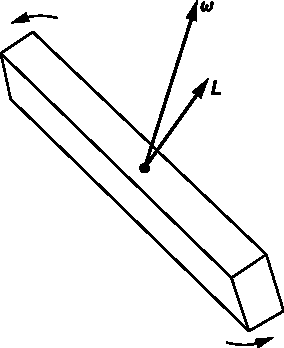
\includegraphics[width=0.5\linewidth]{fyz_fig877.pdf}
      \caption{
              (\cite[s.~707]{Feynman02})}
      \label{fyz:fig877}
    \end{figure}

  \section{Vektorový součin}\label{fyz:IIchapXXXIsecV}
  \section{Tenzor napětí}\label{fyz:IIchapXXXIsecVI}
  \section{Tenzory vyššího řádu}\label{fyz:IIchapXXXIsecVII}
  \section{Čtyřtenzor elektromagnetické energie a hybnosti}\label{fyz:IIchapXXXIsecVIII}
  \section{Příklady a cvičení}\label{fyz:IIchapXXXIsecIX}









    \begin{figure}[ht!] %\ref{fyz:fig878}
      \centering
      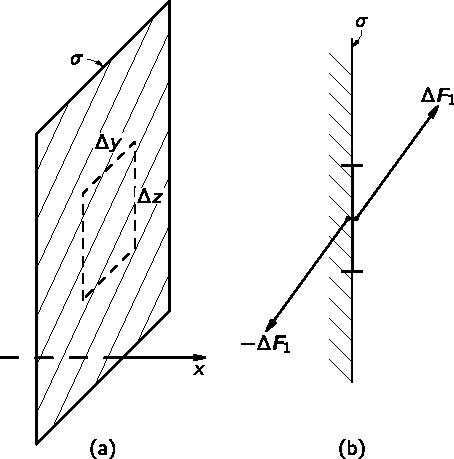
\includegraphics[width=0.7\linewidth]{fyz_fig878.pdf}
      \caption{
               (\cite[s.~707]{Feynman02})}
      \label{fyz:fig878}
    \end{figure}

    \begin{figure}[ht!] %\ref{fyz:fig879}
      \centering
      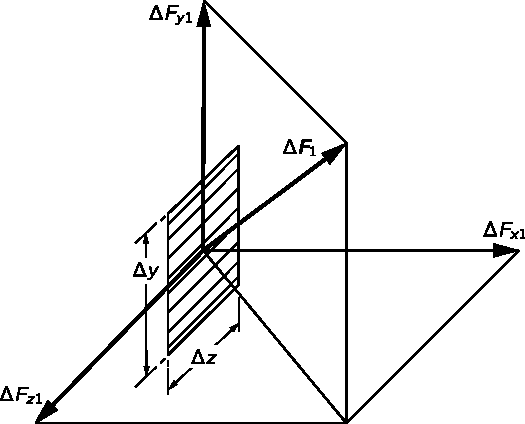
\includegraphics[width=0.7\linewidth]{fyz_fig879.pdf}
      \caption{
               (\cite[s.~707]{Feynman02})}
      \label{fyz:fig879}
    \end{figure}

    \begin{figure}[ht!] %\ref{fyz:fig880}
      \centering
      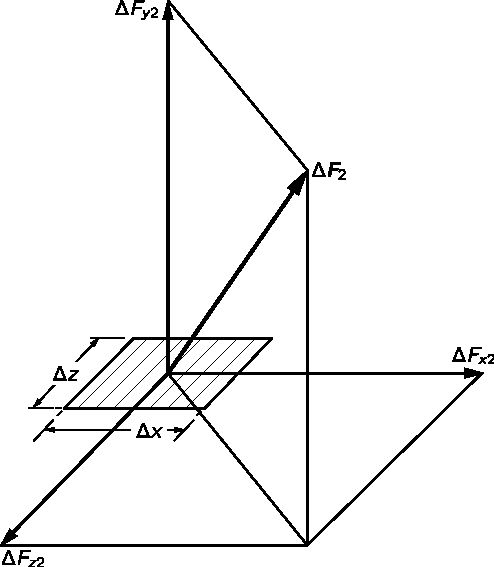
\includegraphics[width=0.7\linewidth]{fyz_fig880.pdf}
      \caption{
               (\cite[s.~707]{Feynman02})}
      \label{fyz:fig880}
    \end{figure}

    \begin{figure}[ht!] %\ref{fyz:fig881}
      \centering
      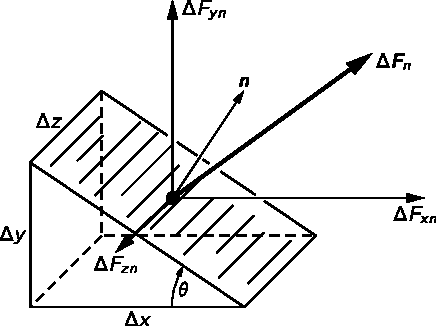
\includegraphics[width=0.7\linewidth]{fyz_fig881.pdf}
      \caption{
               (\cite[s.~707]{Feynman02})}
      \label{fyz:fig881}
    \end{figure}

    \begin{figure}[ht!] %\ref{fyz:fig882}
      \centering
      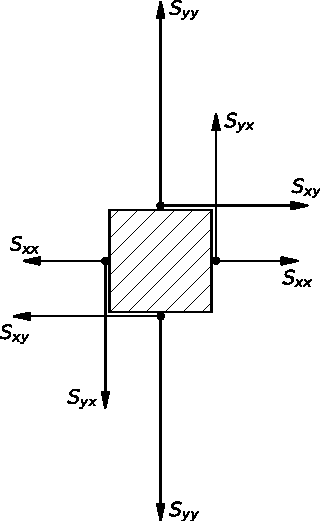
\includegraphics[width=0.7\linewidth]{fyz_fig882.pdf}
      \caption{
               (\cite[s.~707]{Feynman02})}
      \label{fyz:fig882}
    \end{figure}


    \todo[inline]{Kapitola fey2ch31 je nedodělaná, obsahuje pouze obrázky}
%} %tikzset
%---------------------------------------------------------------------------------------------------
